\textbf{\LARGE{Part one: Design Project}}
\todo[inline]{Part one is a design project report as described
    in the coursebook. The audience for this is the companies
    management. See e.g.\ page 186ff.
    Length between 25-30pp}

\section{Objective}

\subsection{Objective of the design project}
\todo[inline]{Quick recap of the requirements from the manager, and what goals 
    the system is designed to fulfill}
The focus of the design project is to improve upon the booking process used by 
\gomonkey. The booking process is currently very manual and only ever handled by 
the manager. The manager said that: 

\begin{quotation}
I don't dare letting my employees handle the bookings.

\em - Michel Pascual, manager and owner of \gomonkey, 15.10.2013
\end{quotation}

He is afraid they will make mistakes, since the process is complex and not very 
well documented. Some bookings may also contain cases which the manager is not 
yet sure of how should be handled, and thus needs an authority to handle and  
produce a best practice for \gomonkey{}. While the manager does spend a lot of
time handling bookings, this takes time from actually evolving the business.
The goal of the design project is to put the booking process into a 
well defined system and reduce the complexity and time required for handling
incoming bookings. This will reduce the workload put on the manager, thus 
empowering him to focus on other areas of the business.

\subsection{Results from the in-line analysis}
The in-line analysis is meant to help us understand the environment in which 
the company is situated, the business strategy of the company, and what work
domains are defined within the business. This will help the designers to
better understand the reasoning behind current work practices and how to 
solve the problems that arise. The most noteable parts of the results from 
the in-line analysis is the business strategy and the overview of the work 
domains of \gomonkey{}.

\subsubsection{Business strategy}
The business strategy of \gomonkey{} was not written down before we started the
project, so we had to construct and interpret on our perception of the company.
This changed during the course of the design project, and this is the final 
result:

\begin{enumerate}
	\item Become a self-sustainable climbing company with customers on a daily basis.
	\item Minimize time requirements pr. booking/customer.
	\item Minimize staff requirements to keep costs low.
	\item Increase sales (Such as selling food and drinks).
	\item Provide better and more comprehensive service than competitors.
\end{enumerate}

\subsubsection{Work domains}
The company, while selling climbing sessions as a service, clearly does other
things that does not directly add value, but a necessary nonetheless.		%this is spelled correctly! nonetheless
While interviewing and observing the company, we mapped out those areas of 
work, and the result can be seen here:

\begin{itemize}
	\item Booking Flow
	\begin{itemize}	
		\item Registering received bookings
		\item Checking payment status
		\item Informing customers prior to arrival
		\item Receiving customers
	\end{itemize}

	\item Employee Schedule
	\begin{itemize}
		\item Scheduling shifts
		\item Swapping shifts
		\item Time registration
	\end{itemize}

	\item Economy and bookkeeping
	\begin{itemize}
		\item Payment during booking
		\item Invoice after visit
	\end{itemize}

	\item Inventory Management
	\begin{itemize}	
		\item Maintenance of inventory
		\item Stock control of equipment
	\end{itemize}

	\item Marketing
	\begin{itemize}
		\item Advertising
		\item Offers and discounts
	\end{itemize}
\end{itemize} 


\subsection{Results from the in-depth analysis}
\todo[inline]{Observations, standard systems, work practices}

The in-depth analysis is meant to help us understand exactly how and why the 
existing processes work as they do. This was done by observing the processes,
analysing documents and correspondance, and mapping out exactly what work 
practices resulted in problematic situations. In the following section we describe the 
work practies we found, and what problems were discovered. When we knew the
business practices and related problemss, we surveyed the market for a useable 
standard system, which is described later in this section.

\subsubsection{Work practices and their problems}

\subsubsection{Finding a suitable standard systems}
It is often a good solution to find a standard system which solves the problem 
at hand. This can save a lot of time and money, and can quickly solve a complex
problem.
We compiled a list of possible standard systems and isolated three very possible
candidates. After deep testing sessions of all systems, we realized that none
of them fulfill the defined requirements in the design project. The testing
session included creating a free temporary booking system. All systems tend to 
have this feature, so potential customers can evaluate the usefullness prior to 
paying. Attempts were then made to setup the system to support the needs of
\gomonkey{}, and after testing the usefullness of the result, we could conclude
upon the advantages and disadvantages of implementing the system.

\begin{description}
\item[SuperSaaS]
We decided not to use SuperSaaS, since the booking doesn’t support the required 
fields for the booking. A 'form' can be attached to a booking after submitting 
initial information (intial information being the date and time of booking, 
name, phone number and email address), and this 
form can include extra information about amount of people in each age group, the
type of customer and food. This information can only be seen with two clicks 
from the calendar overview, thus making it impossible to get a good overview of 
how 'available' a time slot is.

Furthermore, it is not possible to calculate a price based on the custom fields 
in the form, and as such, the system cannot ask for a deposit so we will still 
need another payment processor.

\item[onlinebooq.dk]
The second promising booking system was onlinebooq.dk. They support selling 
'services', but unfortunately they only support selling one of each servive.
This can be seen in \autoref{fig:onlinebooq} as the checkbox, next to the 
service in question. This makes it useless for \gomonkey{}, since the price is 
calculated from the amount of people utilizing each service. It does support 
paypal and quickpay, but this doesn't matter if we cannot calculate the price 
correctly.

\todo[inline]{Remove border around \autoref{fig:onlinebooq}}
\begin{figure}[htbp]
    \centering
        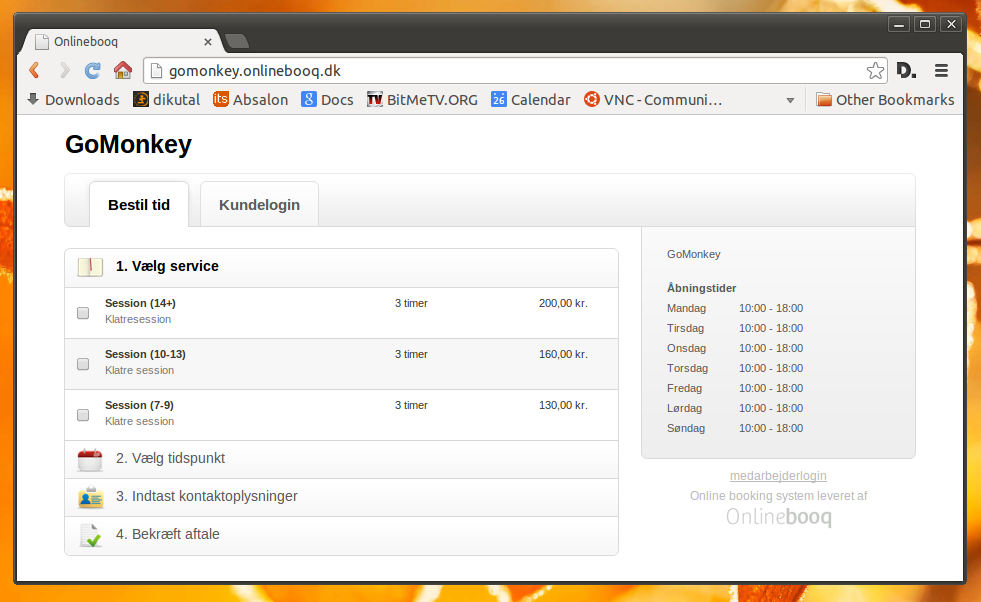
\includegraphics[width=.8\textwidth]{figures/onlinebooq.png}
	    \caption{Screenshot from testing onlinebooq.dk.}
        \label{fig:onlinebooq}
\end{figure}
		

\item[Cyberbooking]
The last booking system we tested was Cyberbooking. They have two types of 
calendars, one which supports one resource (e.g. a hairdresser) who can only
perform one service at a time. The other type supports booking slots on 
predefined events, (e.g. a fitness session) and the events are set by the 
company. None of these types can help \gomonkey{} with the booking process,
since the amount of resources aren't limited to one group of customers, and 
the times of bookings are very flexible.
\end{description}

While none of the systems fit with \gomonkey{}'s business, we attempted
to find a way to adjust \gomonkey{}'s business to the systems. This was not 
successful and would alter the work practices in a very negative way.


\section{The coherent vision}
The coherent vision we suggest here is based on the results from the in-line 
analysis and in-depth analysis. The vision is a suggestion for a system design, 
along with descriptions of any expected organizational additions and changes 
resulting from implemeting the system. It also includes reflections upon 
required qualifications of anyone who will have to interact with the system
and what advantages and disadvantages this will enforce thoughout the company.
Finally, it includes some financial figures and an implementation plan. This 
should give the required knowledge of the system to perform an informed choice
on wether to start the project.

\subsection{Technology and systems}
This section will describe the system itself, what it does and how it looks,
along with what is required to keep the system running.

\subsubsection{IT systems and platform}
\todo[inline]{What do we need for running the system. Servers, software, etc}
The owner of \gomonkey insists that the main website continues to run on the 
WordPress which is hosted with One.com. This is a fine solution, and will make
sure that the website maintains it's current, existing Google page-rank.

Further, we need a server for hosting the new system, which can not be developed
and run on the One.com server. For this, we will need a server with a database
and a webserver. Preferably, a server with root access, but a server with the 
necessary interfaces to the previously mentioned items will be sufficient.

\subsubsection{Functions of the system}
\todo[inline]{Describe what the system does}

\subsubsection{User interaction}
\todo[inline]{Pictures of mockup and descriptions of how it works}

\subsection{Work organization}
\todo[inline]{Do we change how the work organization is, someone with new
responsibilities? Can someone potentially do some of the managers work?}

\subsection{Qualification needs}
\todo[inline]{Does the system require any education? The manager will probably
need to tell about the new system to the instructors, and the manager will have
to be 'taught' how to use the new system.}
	
\subsection{Advantages and disadvantages}
\subsubsection{Business- and IT strategies}
\todo[inline]{How the system will help reach the goals described in the
    business- and IT strategies.}

\subsubsection{Groups of staff and their relations}
\todo[inline]{Advantages and disadvantages from an employees and the managers 
    perspective, and how the it system affects their communication and 
    relation.}

\subsubsection{Customers}
\todo[inline]{Advantages and disadvantages from a customers perspective.}


\section{Finances?}
\todo[inline]{Does this even make sense for the company?}


\section{Implementation strategy and plan}
\subsection{Technical implementation}
\subsection{Organizational implementation}

\section{Recommendations and priorities}

\newpage
